\documentclass[11pt]{ltjsarticle}
%\usepackage[dvipdfmx]{graphicx}
\usepackage{graphicx}
\usepackage{booktabs}
\usepackage{mathcomp}
\usepackage{array}
\usepackage{mathtools,amssymb}
\usepackage{siunitx}
\usepackage{multirow}
\usepackage{tabularx}
\usepackage{subcaption}
\usepackage{float}
\usepackage{abstract}

\title{仮想筋電義手の開発に関する研究}
\author{河合 将暉}
\adviser{戸崎 哲也}

\thispagestyle{empty}
\pagestyle{empty}

\begin{document}
\maketitle

\section{はじめに}
	上肢切断者が筋電義手を装着する際,筋電義手を自在に扱う
	ことができるように訓練を行う必要がある.また,上肢を切断しても
	欠損した部位が存在するかのように錯覚したり,その部位が痛むこと(この痛みを幻肢痛と呼ぶ)
	がある.VRを用いた筋電義手トレーニングの効果については先行研究
	\cite{ref:1}%\cite{ref:2}%
	で検討されているが,仮想筋電義手(Virtual Hand)
	の見た目よっても訓練効果や幻肢痛緩和の有意差があると考られる.
	そのため,本研究では,3Dスキャナを用いて仮想筋電義手のモデルを
	組み込んだ仮想筋電義手トレーニングシステムを構成することを目的とする.
\section{研究内容}
	\subsection{3Dモデルの構成}
		本研究で使用した3Dスキャナは ``EinScan HX''を用いた.出力方法は
		.mtl形式で出力したものをblenderで表面のノイズ部分を除去・補正し
		見た目に違和感のない程度に後処理を行った.そしてそのモデルに対して
		ボーン(3Dモデルの動きを制御するための骨組み)を図\refeq{fig:VRhand}のように配置した.
		\begin{figure}[H]
		\centering
		\begin{minipage}{0.28\columnwidth}
		\centering
		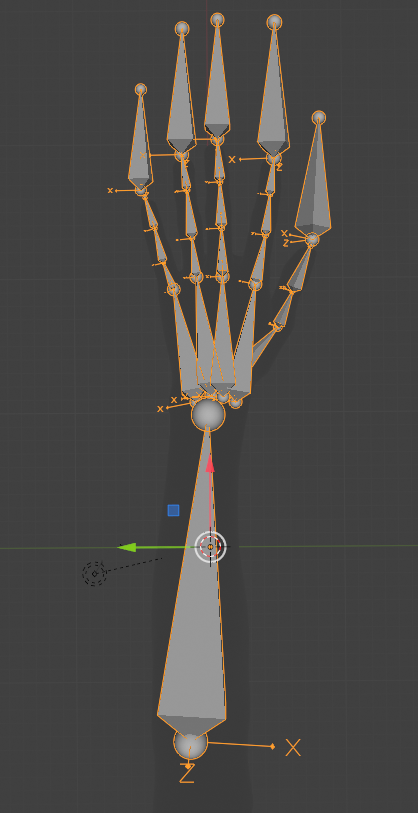
\includegraphics[width = \columnwidth]{figs/handbone.png}
		\subcaption{ボーン構成}
		\end{minipage}
		\hspace{0.1\columnwidth}
		\begin{minipage}{0.4\columnwidth}
		\centering
		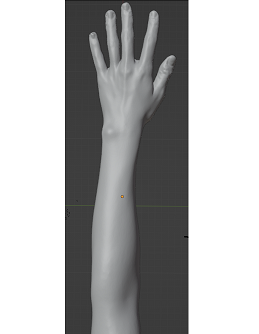
\includegraphics[width = \columnwidth]{figs/handmesh_rear2.png}
		\subcaption{メッシュ構成}
		\end{minipage}
		\caption{仮想筋電3Dモデル構成図}
		\label{fig:VRhand}
		\end{figure}

	\subsection{システムの構成}
		開発環境としてUnityを用いて仮想空間上のトレーニングシステムを構成した.
		仮想空間上のオブジェクトには物理演算をつけており,
		構成した仮想空間には枠組みの中に動かせるオブジェクトとして
		球体・立方体・円錐の3Dモデルを用意し,固定オブジェクトとしては適当な
		高さの長方形3Dモデルを用意した.
		仮想筋電義手モデルはマウスの動きに合わせて前後左右に移動できるように
		構成し,非固定オブジェクトと接触しているときに右クリックを押下している間
		オブジェクトを掴むことができる.

\section{まとめと今後の課題}
	本研究では,筋電義手操作訓練および幻肢痛緩和のための仮想筋電義手
	トレーニングシステムのプロトタイプを構成した.
	今後の課題としては, 腕の動きをVR上に変換するためのインタフェース
	をマウスを用いて構成しているが,実際に上肢切断者を対象として
	シミュレータを扱う場合,マウスを使用できないことを考慮し,
	光変位センサ「First VR」を用いたシステム改善や
	適切なトレーニングシステムの構築および検討を行う予定である.
\begin{thebibliography}{99}%参考文献
	\bibitem{ref:1}
	芝軒 太郎,村上 隆治,島 圭介,辻 敏夫,大塚 彰,陳 隆明:
	``VRを利用した筋電義手操作トレーニングシステム
	の開発と仮想 Box and Block Test の実現'',日本ロボット学会誌,
	vol.30,no.6,pp.621-628 (2012).

	% \bibitem{ref:2}
	% Osumi M, Inomata K, Inoue Y, Otake Y, Morioka S, Sumitani M.
	% Characteristics of Phantom Limb Pain Alleviated with Virtual 
	% Reality Rehabilitation. Pain Med. 2019 May 1;20(5):1038-1046.
	% doi: 10.1093/pm/pny269. PMID: 30576543.
\end{thebibliography}
\end{document}